\chapter{Habitable Worlds}\label{ch:HabitableWorlds}
This chapter was published as
\begin{description}
	\item \fullcite{Lineweaver2012AnnRev}
	%\item Section~\ref{sec:HabEnergies} has been extended.
\end{description}
\section*{Abstract}
We review the habitability of our Earth and other Earth-like planets. Understanding habitability and using that knowledge to locate the nearest habitable planet may be crucial for our survival as a species. To evaluate remotely the habitability of the increasing number of Earth-like exoplanets, we need to understand which features of our own planet enabled the origin and evolution of life – and if these features are universal. We discuss the habitability of Earth, the habitability of planets orbiting other stars, and the habitability of our galaxy. We profile the `bioshell' - the $\sim$\,1\% volume of our planet, which is inhabited by life and describe temperature and nutrient deserts where there is little biomass. The inhabited and uninhabited regions on Earth suggest that the presence of liquid water in a narrow temperature range is the main constraint that can be used in a habitability classification scheme for rocky planets.

We review current ideas about the microbiology and bioenergetics of the earliest terrestrial life forms and find that the conditions for life's emergence may be different and more specific than the broader conditions to which life can adapt. Since life and its environment co-evolve, we propose the dynamic concept of an `Abiogenesis Habitable Zone', where life can get started and which, upon continual modification by life, transitions into a 'Habitable Zone'. Our compilation of recent exoplanet detections suggests that the fraction of stars with planets is $\sim$\,100\% and the fraction of stars with a rocky planet in the habitable zone could be comparably large. Recent discoveries suggest that there are at least 10 times as many Earth-sized planets as Neptune sized planets, which in turn are 10 times more abundant than Jupiter-sized planets. Although the process of rocky planet formation and supply of water to terrestrial planets, seems to be a common product of star formation, the water content of a rocky planet is probably highly variable. This variability can be used to classify their habitability, e.g., ocean planets, Earth-like planets, and desert planets.

\clearpage

\begin{flushright}
		\textit{The Sun with all those planets revolving around it\\ and dependent on it, can still ripen a bunch of grapes\\ as if it had nothing else in the universe to do. \\
		--- Galileo Galilei}
	\end{flushright}

The universe is filled with stars like our Sun \cite{Robles2008}, rocky planets like our Earth \citep{Howard2012}, water like in our oceans \citep{Mottl2007}, amino acids like those that make up our proteins, and all the other ingredients for life \citep{Pizzarello2007}. But is the universe filled with anything we would recognize as life \citep{Lineweaver2006}\,? \citet{DeDuve1995} has argued that the initial deterministic nature of proto-biochemistry makes life a ``cosmic imperative'' built into the chemistry of the universe, and we should therefore expect life to be common in the universe.

%%%%%%%%%%%%%%%%%%%%%%%%%%%%%%%%%%%%%%%%%%
\begin{figure}[!hbt]
	\centering
	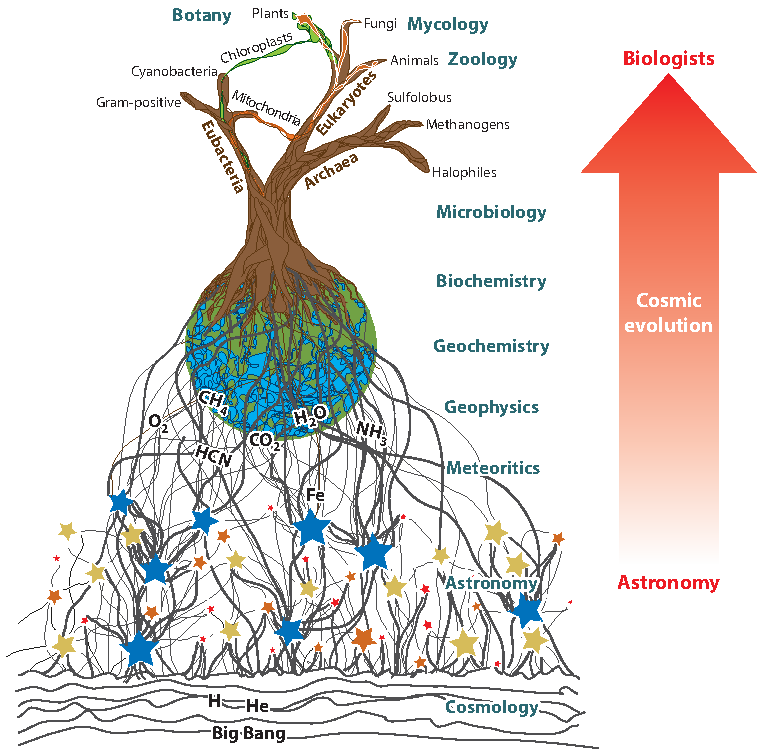
\includegraphics[width=1\linewidth]{figures/AnnRevs/AR1.pdf}
	\caption[Cosmic Evolution]{The emergence of biologists from astronomy. Starting from the big bang at the bottom, deterministic physical sciences set the context for the emergence of life. The resulting biologists (animals) at the top of the tree \citep[\eg][]{Pace1997, Hedges2009} have constructed the brown phylogenetic tree based on the molecular fossils inside the DNA of the inhabitants of the biosphere. The terrestrial tree of life took root approximately four billion years ago. We review the features of rocky planets that are implicated in the ability to give root to, and maintain, a tree of life. 
	}
	\label{fig:AR1}
\end{figure}

%%%%%%%%%%%%%%%%%%%%%%%%%%%%%%%%%%%%%%%%%%
\begin{figure}[!hbt]
	\centering
	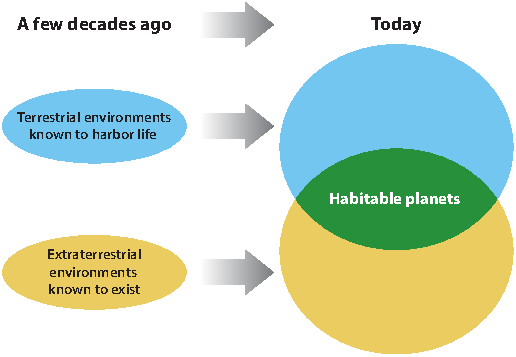
\includegraphics[width=1\linewidth]{figures/AnnRevs/AR2.pdf}
	\caption[Emergence of habitable planets.]{Emergence of habitable planets. Habitable planets are emerging from the increasing overlap of two sets of environments: the increasingly large set of terrestrial environments known to harbor life and the increasingly large set of extraterrestrial environments on the newly detected rocky exoplanets. The overlap of these research fields bolsters expectations that the universe may be filled with habitable planets.}
	\label{fig:AR2}
\end{figure}

Terrestrial life emerged from nonlife approximately four billion years ago \citep{Battistuzzi2004,Sleep2008} (Figure~\ref{fig:AR1}). Descriptions of where this happened include warm little ponds \citep{Darwin1871}, hot hydrothermal vents \citep{Wachtershauser2006, Martin2008}, and cold little ponds \citep{Bada1994}. Scenarios for how life emerged include a prebiotic soup under a reducing atmosphere \citep{Oparin1924, Miller1953} and some form of semi-deterministic molecular chemistry \citep{Dyson1999, Segre2000} that evolved into auto-catalytic reactions \citep{Eigen1971} and produced replicating molecules \citep{Cairns-Smith1982, Gesteland1999}, proto-metabolisms \citep{Pascal2006}, and cell membranes \citep{Deamer2010}. Despite the variety of these scenarios, some common threads represent our best estimates of what we might expect to share with extraterrestrial life. We can expect extraterrestrial life to be based on Darwinian evolution and the most fundamental features of terrestrial biochemistry \citep{Feinberg1978, Pace2001, Morris2003, Benner2004, DeDuve2007, Lineweaver2012}. Noncoincidentally, these are the same features that are often used to define life \citep[\eg][]{Schrodinger1944, Sagan1970, Joyce1994, Leach2006}.
 
During the past few decades, the exploration of some extreme environments on Earth has uncovered extremophile microbial life in conditions previously thought to be too hostile for life. These discoveries have expanded the variety of terrestrial environments known to harbor life \citep{Rothschild2001, Stetter2006, Shock2007, Baross2007, Madigan2010, Pedersen2010}. During the same few decades, progress in the characterization of the planets and moons of our Solar System, and progress in the detection of a wide variety of exoplanets in orbit around an increasingly large fraction of stars, has broadened the range of known extraterrestrial environments (Sections \ref{sec:FractionPlanets} and \ref{sec:HabitableTemperatures}). The growing overlap of these two sets of environments suggests that habitable planets are abundant (Figure~\ref{fig:AR2}). This increases the probability of finding some kind of extraterrestrial life.

The number of papers and conferences reporting new exoplanet and extremophile discoveries, and those grappling with the issue of planetary habitability, has enormously increased. Recent reviews of habitability include \citet{Kasting2003}, \citet{Gaidos2005}, \citet{Hoehler2007a}, \citet{Fishbaugh2007}, \citet{Kopparapu2013} and \citet{Kasting2014}.

This review provides an overview of habitability and focuses on what we know about the habitability of Earth, the habitability of planets orbiting other stars, and the habitability of our galaxy. It synthesizes facts and current ideas about the microbiology of the earliest terrestrial life and the latest findings of planet hunters. It is organized as follows: Section \ref{sec:HZones} reviews the limits of terrestrial life and illustrates where life is found, and is not found, on the habitable planet that we know best—Earth. We discuss energy constraints on life and how the conditions for life's emergence may be different and more specific than the broader conditions to which life can adapt. Section \ref{sec:FractionPlanets} presents the increasingly compelling evidence that planets in general, and rocky planets in particular, are a common product of star formation. Section \ref{sec:HabitableTemperatures} discusses the habitability of the most Earth-like exoplanets and the traditional circumstellar habitable zone (HZ). Section \ref{sec:WaterDel} reviews the supply of water to terrestrial planets. Finally, Section \ref{sec:GHZ} reviews work on the galactic HZ and discusses a variety of habitability issues.

\clearpage
\section{The Habitable Zones on Earth}\label{sec:HZones}
Because habitability is about the complex relationship between life and environment, we start close to home with a discussion of the relationship between terrestrial life and terrestrial environments. The close fit between our requirements and what Earth can provide is not coincidental. Earth and the life on it have coevolved. However, life is not infinitely adaptive. Some parts of Earth are habitable and some, even after approximately four billion years of evolution, are not. Life as we know it has limits, and we can explore these limits most easily on Earth.

%%%%%%%%%%%%%%%%%%%%%%%%%%%%%%%%%%%%%%%%%%
\begin{figure}[!hbt]
	\centering
	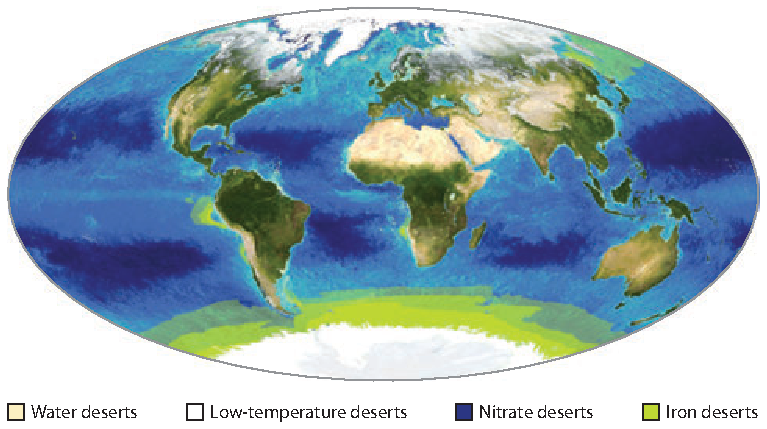
\includegraphics[width=0.9\linewidth]{figures/AnnRevs/AR3.pdf}
	\caption[Deserts on Earth]{Four deserts on Earth's surface. Life is not evenly distributed over the surface of Earth. There are water deserts (sandy brown), low-temperature deserts (white), nitrate deserts (dark blue), and iron deserts (light green), where the abundance of life is significantly lower than in surrounding regions. This map was constructed with data from \citet{Stockli2005,McClain2006}.}
	\label{fig:AR3}
\end{figure}

In a specific region, when some requirement for life is outside the optimal range for life, the total biomass in that region is low (Figure~\ref{fig:AR3} presents these regions). We generically call such regions deserts. Low rainfall makes water deserts. Low temperatures make low-temperature deserts at Earth's poles. Far from land, in mid-oceanic gyres (where windblown dust and aerosols are at a minimum \citep{Duce1991}), low nitrate levels produce nitrate deserts. 

Chlorophyll maps of the ocean \citep{McClain2006,McClain2009} show regions where, despite ample water, photons, and nitrates, there are low concentrations of chlorophyll. Iron fertilization experiments in these enigmatic high-nitrate-low-chlorophyll regions found that the biomass was iron limited, rather than phosphate limited or limited by some other nutrient \citep{Falkowski1998, Smetacek2008}. Such iron deserts have been identified in the Southern Ocean, the northwest Pacific, and the eastern equatorial Pacific. Low-phosphate regions overlap significantly with nitrate deserts \citep{Garcia2006}. Because the elements H, O, C, N, P, and S make up $\sim$\,98\% (by mass) of life \citep{Lineweaver2012}, one might expect analogous C and S deserts.

The subtle variations of biomass over the horizontal surface (Figure~\ref{fig:AR3} ) are dwarfed by the nonsubtle variations of biomass in the vertical direction. The terrestrial biosphere is a thin bioshell whose thickness ($\sim$\,10 km) is $\sim$\,1/600 of Earth's $\sim$\,6,400 km radius. Figure~\ref{fig:AR4}  is a vertical profile of terrestrial biomass. Low temperatures and low densities prevent life from living permanently in air or on the highest mountains (low-temperature deserts). High temperatures prevent life from existing more than $\sim$\,5 kilometers underground, because the average continental geothermal gradient of 20{-}30\textcelsius per km reaches the upper temperature limit of life (122\textcelsius{}, \citep{Takai2008}) at approximately that depth. (Shield gradients and those above subduction zones can be as low as $\sim$\,$10$\textcelsius{} per km.) Thus, the interior of Earth is a spherical high-temperature desert. The bioshell is thin because life is kept squeezed into a narrow HZ between a high-temperature desert below and a low-temperature desert above (Figures \ref{fig:AR4} and \ref{fig:AR5}). 

%%%%%%%%%%%%%%%%%%%%%%%%%%%%%%%%%%%%%%%%%%
\begin{figure}[!hbt]
	\centering
	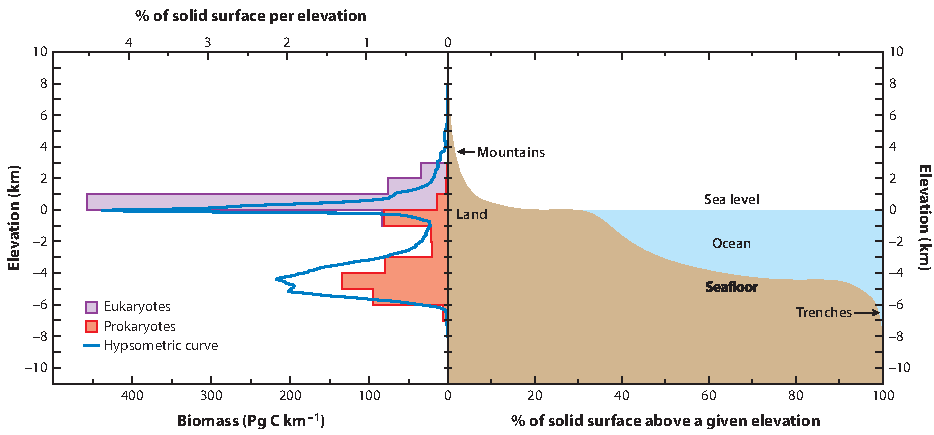
\includegraphics[width=0.9\linewidth]{figures/AnnRevs/AR4.pdf}
	\caption[Terrestrial bioshell]{Vertical profile of biomass in the thin terrestrial bioshell ($\pm$10 km). The hypsographic curve on the right shows the fraction of Earth's solid surface above a given elevation. For example, 30\% of the solid surface is above sea level, whereas the remaining 70\% is below sea level. The hypsometric curve on the left (blue line) \citet{Perotti2011} shows the fraction of Earth's solid surface at any given elevation. The histogram on the left shows our estimate of the vertical profile of terrestrial biomass (total carbon in terrestrial life forms) derived from combining data from \citet{Whitman1998,Houghton2003}. Since the publication of the paper presented in this chpater, \citet{Kallmeyer2012} analysed a more diverse range of sediment samples and estimate that the biomass in sub-seafloor sediments is 10-45\% lower than estimates used by \citet{Whitman1998}. \citet{Jorgensen2012,Hinrichs2012} and further analysis by \citet{Mcmahon2014} confirm the overestimation by \citet{Whitman1998}. However, we find that even with the new estimates our main conclusions of the relative distribution of prokaryotic and eukaryotic life is not challenged.}
	\label{fig:AR4}
\end{figure}

%%%%%%%%%%%%%%%%%%%%%%%%%%%%%%%%%%%%%%%%%
\begin{figure}[!hbt]
	\centering
	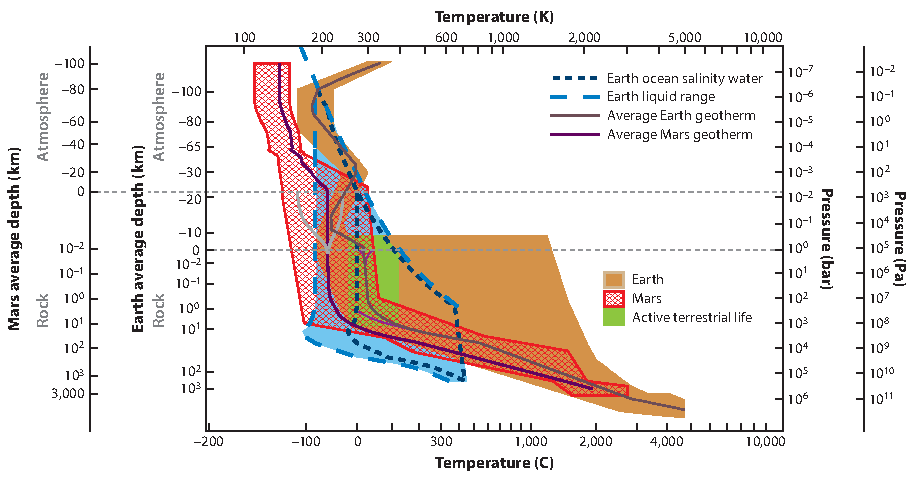
\includegraphics[width=0.9\linewidth]{figures/AnnRevs/AR5.pdf}
	\caption[Uninhabited water on Earth \& Mars]{Uninhabited water on Earth and the potential biosphere of Mars. This pressure-temperature phase diagram is a superposition of the region where H$_{2}$O is liquid (blue), all terrestrial environments (brown), inhabited terrestrial environments (green), and all Martian environments (hatched red). Notice the large regions of uninhabited terrestrial liquid water that is either too cold ({-}80\textcelsius{} < T < {-}20\textcelsius{}) or too hot (122\textcelsius{} < T < 400\textcelsius{}) for life. The $\pm$10 km vertical extent of the green area corresponds to the elevation range of the biomass profile in Figure~\ref{fig:AR4}. The shape of the green area shows that the presence of liquid water and the {-}20\textcelsius{} to {+}122\textcelsius{} temperature range are the dominant variables determining habitability. These inhabited and uninhabited terrestrial environments, set by the need for liquid water and a specific range of temperature, are our best guides to exoplanet habitability. Figure from \citet{Jones2011}. See also \citet{Mottl2007,Jones2010,Jones2012,Cockell2011}.}
	\label{fig:AR5}
\end{figure}

Terrestrial biomass is approximately evenly divided between eukaryotes (55\%; Figure~\ref{fig:AR4}, light purple) and prokaryotes (45\%; Figure~\ref{fig:AR4}, orange). Biomass is also roughly evenly divided between above sea level (56\%) and below sea level (44\%). Of Earth's eukaryotic biomass, 99.5\% is on land \citep{Sundquist2014}. About 96\% of prokaryotic biomass is below sea level, mostly in seafloor sediments \citep{Whitman1998}. The oxygenic photosynthesis that powers most of the eukaryotic life on land was a relatively late adaptation \citep{Kiang2007, Sleep2007}, as was the ability to colonize the land \citep{Battistuzzi2004}. Five hundred million years ago, there was land but little eukaryotic life on it. Thus, for approximately the first three billion years, the profile of terrestrial biomass may have resembled the current prokaryotic profile (Figure~\ref{fig:AR4}, orange).

\subsection{The Abiogenesis Habitable Zone}
As we learn more about the origin of life, we can start to define an abiogenesis habitable zone (AHZ) where the requirements for life's emergence are met. The habitability requirements for the origin of life may be substantially different from, and more specific than, the requirements to maintain life on a planet—think of the difference between a spark plug to start an engine and a carburetor to supply it with fuel. If you shine light onto a vat of HOCNPS, or bubble molecular hydrogen through a flask of amino acids, life does not spontaneously emerge. For a planet to manage the transition from the nonliving to the living\,-\,to qualify as an AHZ\,-\,juxtapositions and flows of specific combinations of molecules are needed to produce auto-catalytic reactions and proto-metabolisms that can tap into either the flow of redox pairs or photons \citep{DeDuve1995, Lane2010}.

Once life begins, organisms do not just passively adapt to preexisting environments. They actively change and construct the world they live in \citep{Odling-Smee2003}. The evolutionary history of life on Earth can be written in terms of how organisms have modified their environments. From the oxygenation of the atmosphere to the creation of beaver dams, life modifies its environment. But life also modifies itself and adapts to fit the environment—evolving, for example, spores to survive dry conditions, antifreeze for survival at low temperatures, and salt pumps to survive at high salinity. Whether life adapts to fit an environment or modifies an environment to be able to survive, the result is the same: The initial specific AHZ is widened (Figure~\ref{fig:AR6}). Through its management of the greenhouse and its partitioning of reductants and oxidants, the activity of life increases the range of inhabited environments \citep{Nisbet2007,Hazen2008}. 

%%%%%%%%%%%%%%%%%%%%%%%%%%%%%%%%%%%%%%%%%%
\begin{figure}[!hbt]
	\centering
	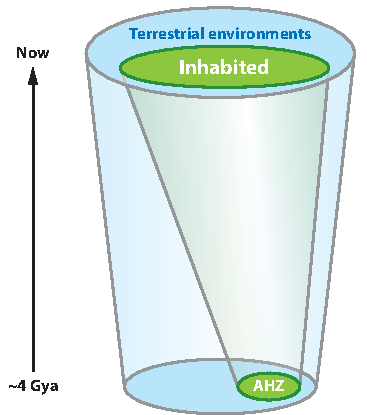
\includegraphics[width=0.5\linewidth]{figures/AnnRevs/AR6.pdf}
	\caption[Abiogenesis habitable zone]{Abiogenesis habitable zone (AHZ). The conditions needed for the origin of life (before life could adapt) are narrower than the broader conditions to which life can adapt.}
	\label{fig:AR6}
\end{figure}

Environments change life-forms, and life-forms change environments. This feedback between life and environment may be so strong that, for a planet to be habitable, it might have to be inhabited. Thus, planetary habitability becomes a dynamic concept with different stages. Habitability begins as a relatively narrow AHZ, completely dependent on the chemistry and other physical characteristics of the planet. Once life emerges and passes the ``Darwinian threshold'' \citep{Woese2002} habitability shifts to a dependence on both the characteristics of the planet and the adaptability of its life-forms. Finally, habitability becomes predominantly dependent on the ability of the inhabitants to regulate their environment. The thermoregulation of Earth over the past four billion years, despite a 30\% increase in solar luminosity, is a possible example of such Gaian regulation \citep{Lovelock1965,Lovelock2000,Lovelock1974,Schneider1991,Schneider2004}. It may be that natural negative-feedback processes, such as the carbon-silicate cycle \citep{Walker1981}, without Gaian regulation, are not conducive to life any more than a nonevolving body would be \citep{Schwartzman1989}. Thus, eventually, habitability becomes a property of life, as much as, or perhaps more than, it is a property of a planet.

The persistence of life on Earth requires liquid water, an appropriate temperature range, nutrients, and an energy source. Self-assembly is an example of an additional requirement for abiogenesis that would be relaxed once life got started (making the AHZ narrower than the HZ). For example, origin-of-life chemists are trying to understand how RNA could self-assemble in the presence of water \citep[\eg][]{Szostak2001}. To self-assemble, dehydration reactions are needed. Cyclic evaporative dehydration could happen near continental hot springs or in warm tidal pools as the kilometer-high tides came in and out every few hours \citep[\eg][]{Lathe2004}. On ocean planets (Section \ref{sec:HabitableTemperatures}), there could be no dehydration reactions because there would be no evaporation from solid surfaces. Thus RNA would not self-assemble and life might not be able to get started on ocean planets. If the self-assembly of RNA required cyclic evaporation, and this assembly was critical to the emergence of life, ocean planets would be lifeless. They would be habitable but uninhabited planets.

\subsection{Habitable Energies}
\label{sec:HabEnergies}
On Earth today, $\sim$\,60\% of the biomass is phototrophic and $\sim$\,40\% is chemotrophic (Figure~\ref{fig:AR4}). Thus, the dominant energy source for life is the solar photon flux. However, when life emerged approximately four billion years ago there may have been much less dry land \citep{Taylor2009} and no eukaryotes. The terrestrial biomass distribution thus may have more closely resembled the current prokaryotic distribution in which the majority of the biomass is not necessarily in the photic zone but at hydrothermal vents at various depths, which were more common approximately four billion years ago \citep{Southam2007,Sleep2010}. Studying the earliest and most fundamental metabolisms of terrestrial life is our best hope for understanding how likely such energy-transducing metabolisms (and thus life) are to emerge elsewhere. Candidates for the earliest metabolisms include two broad categories of primary producers: anoxygenic phototrophs and chemolithotrophs. Chemolithotrophs live off inorganic redox pairs supplied by chemical disequilibria at hydrothermal vents \citep{Nisbet2001,Kelly2006}.

%%%%%%%%%%%%%%%%%%%%%%%%%%%%%%%%%%%%%%%%%%
\begin{figure}[!hbt]
	\centering
	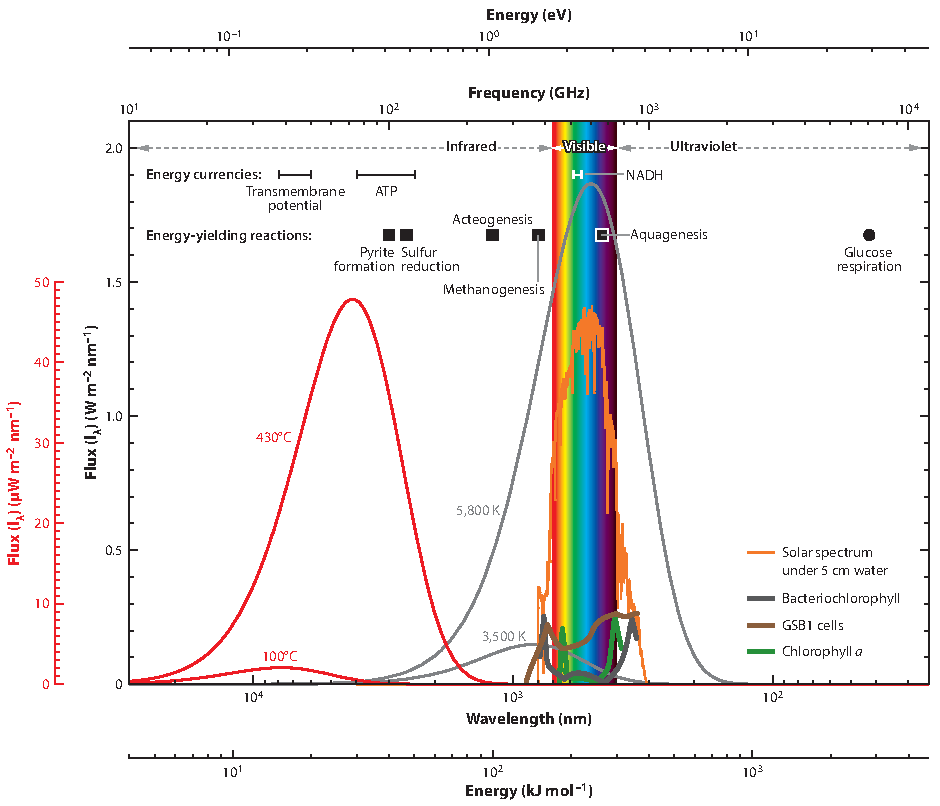
\includegraphics[width=0.9\linewidth]{figures/AnnRevs/AR7.pdf}
	\caption[Energy sources and currencies of life]{Comparison of the photon and redox energy sources of early life with the dominant energy currencies of life. The two sources of energy available to early life were solar photons (represented by the solar spectrum as seen from beneath 5 cm of water (orange)) and inorganic redox pairs available at hydrothermal vents (black squares). The energy obtained from both these sources was converted into the currencies life uses to store or circulate energy (transmembrane potential, ATP, and NADH). Uncertainties indicate the common range of energies associated with these currencies under physiological conditions. Five redox reactions are shown that are candidates for the sources of energy for the first chemolithotrophs (see Table \ref{tab:energycurreny} and \citet{Blank2009}). Blackbody curves are shown for Sun-like G stars and for the most common star in the universe, low-mass M stars such as Gl581 (Section \ref{sec:HabitableTemperatures}). On the left, using a different y-axis, the blackbody spectra of a 430\textcelsius{} hydrothermal vent (or hot spring) fluid and a 100\textcelsius{} fluid represent the native environment of hyperthermophiles. Absorption spectra are shown for two candidates for the earliest anoxygenic photosynthesis: bacteriochlorophyll \citep{Frigaard1996,Madigan2006} and the spectra of intact cells of an obligately photosynthetic bacterial anaerobe (green sulfur bacterium, GSB1) isolated from a deep-sea hydrothermal vent environment \citep{Beatty2005}. The absorption spectrum of eukaryotic chlorophyll a \citep{Cinque2000} and the maximum energy available from oxic glucose respiration are shown for comparison.}
	\label{fig:AR7}
\end{figure}

\begin{table}[!hbt]
	\centering
		\caption[Redox energy currencies and reactions]{Free energies ($\bigtriangleup$G) of redox chemistry of some of the earliest terrestrial energy yielding reactions plotted in Figure~\ref{fig:AR7} \citep{Amend2001,Martin2008,Chang2005,Nicholls1992}. Oxic respiration of glucose is included for comparison.}
	\resizebox{\textwidth}{!}{%
		\begin{tabular}{@{}llcccc@{}}
			\toprule
			{Energy currency} & & {$\bigtriangleup$G (kJ/mol)}  & {Example} \\ \midrule
			Trans-membrane potential                &               & 12-20   & all organisms                                                      \\
			ATP                             &                       & 30-50   & all organisms                                                      \\
			NADH                           &                        & 210-220 & all organisms                                                      \\ \bottomrule
			\\ \toprule
					{Energy yielding reaction} & & {$\bigtriangleup$G (kJ/mol)}  & {Example} \\ \midrule
			FeS(s) + H$_{2}$S(g) $\rightarrow$ FeS$_{2}$(s)+ H$_{2}$(g) &pyrite formation      & 40        & Iron-sulphur world \citep{Wachtershauser1998}                                                \\
			S(s) + H$_{2}$(aq) $\rightarrow$ H$_{2}$S(aq) &sulphur reduction              & 45        & \textit{Sulfurospirillum}, \textit{Pyrodictium occultum}, \textit{Thermococuss} spp.          \\
			4H$_{2}$(aq) + 2CO$_{2}$(aq) $\rightarrow$ CH$_{3}$COOH(aq) + 2H$_{2}$O(l) &acetogenesis & 100       & \textit{Acetogenium kivui}, \textit{Acetobacterium} spp., \textit{Clostridium thermoaceticum} \\
			CO$_{2}$(aq) + 4H$_{2}$(aq) $\rightarrow$ CH4(aq) + 2H$_{2}$O(l) &methanogenesis   & 130       & \textit{Methanococcus}, \textit{Methanobacterium}                                    \\
			H$_{2}$(aq) + 0.5CO$_{2}$ (aq) $\rightarrow$ H$_{2}$O(l)&aquagenesis               & 250       & \textit{Aquifex aeolicus}                                                  \\
			C$_{6}$H$_{12}$O$_{6}$ + O$_{2}$ $\rightarrow$ CO$_{2}$ + H$_{2}$O &oxic respiration              & 2870      & Many bacteria, archaea and eukaryotes including \textit{Homo sapiens}    \\ \bottomrule 
		\end{tabular}
	}
	\label{tab:energycurreny}
\end{table}



Hyperthermophiles are the deepest- and shortest-branched organisms on the phylogenetic tree of life \citep[\eg][]{Pace1997, Lineweaver2003}. Hyperthermophiles gain energy by inorganic redox reactions employing compounds such as H$_{2}$, CO$_{2}$, S$^{0}$, Fe$^{2+}$, and Fe$^{3+}$ \citep{Stetter2006}. Redox reactions in hydrothermal vents and hot springs probably played a dominant role in early metabolism. The earliest life forms were probably chemoheterotrophs that evolved in high-temperature, low-pH, and high-salinity environments resembling hydrothermal vents \citep{Martin2008} or hot springs. The transition of life from a redox-only energy source to a redox and photon energy source is suggested by comparing the energies of different metabolic reactions in Figure~\ref{fig:AR7} \citep{Sleep2008}. The earliest redox reactions -- pyrite formation, sulfur reduction, methanogenesis, and acetogenesis \citep{Wachtershauser1998,Martin2007,Blank2009,Ljungdahl1986} -- provide less energy than photosynthesis. However, these early reactions do provide enough energy to charge transmembrane potentials in a chemiosmotic coupling and convert low-energy molecules such as ADP, NAD$^{+}$, and NADP$^{+}$ to higher-energy molecules such as ATP, NADH, and NADPH \citep{Mitchell1961}. These molecules are universal energy currencies and likely to have been adopted by the earliest organisms.
 
Energy sources based on a redox gradient may have been ubiquitous on the early Earth, particularly because hydrothermal activity may have been more widespread than it is today \citep{Sleep2007}. The similar energies of the earliest metabolic pathways and the availability of the reactants in environments such as hydrothermal vents bolster the case that life began by using energy sources based on redox gradients and over time evolved to perform higher-energy reactions such as oxygenic photosynthesis and oxic respiration. \citet{Canfield2006} claim that the most-active, earliest ecosystems were probably driven by the cycling of H$_{2}$ and Fe$^{2+}$ through primary production conducted by anoxygenic phototrophs.

The absorption spectra of bacteriochlorophylls, which are considered to be more ancient than chlorophylls \citep{Hohmann-marriott2011,Blankenship2010}, and the photosynthetic pigments in green sulfur bacterium (GSB1) peak outside the visible region of the spectrum in the near-IR, where photons can penetrate to some degree through murky water. Although the blackbody emission of hot hydrothermal fluids has far fewer photons in the near-IR than in the mid-IR, they are in sufficient numbers and of high enough energy that GSB1 can photosynthesize and live in a dark environment. Photons of even lower energies ($\sim$\,1,000 nm) are used by purple anoxygenic bacteria \citep{Kiang2007}. Note that all redox reactions in Figure~\ref{fig:AR7} are above the peak energy of the 100\textcelsius{} ambient temperature of a hyperthermophile environment. Any redox reaction that is used by life must satisfy the constraint that the activation energies must be higher than what is available as background energy in the environment \citep{Shock2007}. An upper limit for the temperature at which metabolic activity can take place is set by the temperature at which the molecular dissociation of proteins and membranes takes place.

%%%%%%%%%%%%%%%%%%%%%%%%%%%%%%%%%%%%%%%%%%
\begin{figure}[!hbt]
	\centering
	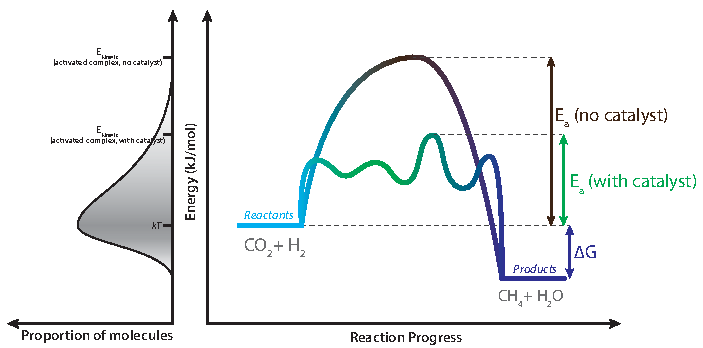
\includegraphics[width=1\linewidth]{figures/Reactions.pdf}
	\caption[Thermodynamics of energy sources for life]{The relationship between environmental kinetic energy kT (represented by the Maxwell-Boltzman distribution on the left), and energies associated with chemical reactions (on the right). Any metabolic reaction used by life must have activation energies higher than kT (the average energy of reactant molecules and the environment) otherwise the reaction would proceed to equilibrium without being mediated by the bio-catalysts of life \citet{Shock2007}. Life makes a living by developing bio-catalysts to lower the activation energy of the reactions of available redox pairs. Metabolism is based on the ability to control the presence of these bio-catalysts \citet{Nealson1999}. Life elsewhere could extract energy from a variety of abiotically produced chemical disequilibria since both the ingredients and the free energy sources (redox or photon based) should be available at the atmosphere:rock-surface or the ocean:rock-surface interfaces on Mars, Titan, Europa and other exoplanetary systems.}
	\label{fig:Reactions}
\end{figure}

If solvents are required for biochemistry, then the temperature at which the solvent remains a liquid, will set the energies of the reactions that biological catalysts can control (Figure~\ref{fig:Reactions}). Typically in terrestrial biochemistry, E$_{a}$(no catalyst) / E$_{a}$(with catalyst) is greater than 10, so the choice of catalyst provides a strong control of the reaction rate \citep{Quinn2014,Alberty2005}. When life was first emerging on Earth and the first catalysts were evolving, this ratio must have been $\sim$\,1, and then gradually evolved to the much larger values (10\,-\,30) that are typical of catalysts used by biota today. 

Energy sources based on redox gradients should be plentiful on rocky planets in circumstellar habitable zones because of the ubiquity of differentially oxidised minerals in the presence of water heated by radiogenic or convective sources in the first approximately 0.5 to 1 billion years of an active wet rocky planet. Over time, life would evolve new catalysts that give access to a wider range of redox pairs and photons, plausibly resulting in a remotely detectable atmospheric biosignature.

If the conditions that permitted terrestrial abiogenesis based on energy-yielding metabolic reactions, such as those plotted in Figure~\ref{fig:AR7}, are not available on other planets, then the search for life elsewhere in the universe may yield the discovery of numerous habitable planets that have remained uninhabited. This is one possible outcome of Mars exploration. The search for life elsewhere in our Solar System has focused on Mars because it is relatively close and because Mars probably contains a lot of subsurface water \citep{Jones2011,Michalski2013}. In Figure~\ref{fig:AR5}, the substantial overlap of the green and red areas represents extensive water at habitable temperatures on Mars. This, combined with much other evidence for water on Mars, suggests that we will find liquid water in the Martian subsurface at temperatures compatible with terrestrial life. If appropriate redox pairs exist, psychrophilic terrestrial life should be able to live between tens of centimeters and ten kilometers beneath the Martian surface \citep{Jones2011}. However, Mars exploration has not yet found any life. In 1976, two Viking spacecraft landed on Mars with life-detection instruments, which returned ambiguous results that have been interpreted as offering no evidence for life \citep{Klein1979,Klein1999,Navarro-Gonzalez2010} \citep[see, however,][]{Levin1981}. Although the Viking mission only attempted to search for active life on the surface (and not in the region below 10 cm where liquid water might be present), there are other potential biosignatures of subsurface life that may be detectable on the surface. One such potential biosignature was recently detected as transitory faint traces of methane \citep{Formisano2004,Krasnopolsky2004,Mumma2009,Lefevre2009}. The debate about whether this methane could be biotic or abiotic seems to be leaning toward an abiotic explanation: Hot olivine exposed to water and CO$_{2}$ undergoes serpentinization and produces methane \citep{Kasting2012,Webster2011}.

NASA's Mars Science Laboratory (MSL), launched on November 26, 2011, has 10 instruments to help determine if life did, or does, exist on Mars. The ongoing exploration of the Martian subsurface is one of the most promising fields where progress in our understanding of habitability can be made. For example, MSL recently detected trace amounts of methane in the Martian atmosphere (in the parts per billion by volume range). The transient spikes in methane abundance suggest episodic production of methane possibly from extant methanogenesis or released from past reservoirs, or both \cite{Webster2015}. Other promising destinations include Jupiter's moons Europa, Ganymede, and Callisto and Saturn's moons Titan and Enceladus. These large moons may have provided wet incubators where life could have emerged (and might still exist). Evidence from the Galileo mission \citep{Spohn2003} suggests that Europa, Ganymede, and Callisto contain a combined volume of liquid water 30–35 times that of Earth's oceans. For reviews of the habitability of our Solar System, see \citet{Shapiro2009} and \citet{McKay2011}. There are also specific papers on the habitability of Europa \citep{Chyba2001,Hand2007}, Enceladus \citep{McKay2008}, Titan \citep{Benner2004,McKay2005,Raulin2008}, and Venus \citep{Grinspoon1997,Svedhem2007}.

\clearpage

\begin{flushright}
	\textit{Since stars appear to be suns, and suns, according to the common opinion, are bodies that serve to enlighten, warm, and sustain a system of planets, we may have an idea of the numberless globes that serve for the habitaton of living creatures.\\
		--- William Herschel}
\end{flushright}

\section{What fraction of stars have terrestial planets}\label{sec:FractionPlanets}

Outside our own Solar System, terrestrial planets or large rocky moons in the circumstellar HZs around other stars are the most likely habitable places. Since 1995, when the first exoplanet was detected around a Sun-like star \citep{Mayor1995}, the fraction of stars with planets has been periodically reported. These are listed in Table \ref{tab:fracstars} and plotted in Figure~\ref{fig:AR8}. The values depend on what fraction of the mass-period parameter space of Figure~\ref{fig:AR9} has been sampled or extrapolated over. Because no technique can sample the entire space, coverage is always incomplete and any reported value such as ``10\% of stars have planets'' is a lower limit—the actual value is larger. Because of this incompleteness, the data are, and always have been, consistent with 100\% of stars having planets. This is represented in Figure~\ref{fig:AR8} by the blue arrows extending from the reported lower limits to 100\%. See \citet{Cassan2012} for supporting evidence from microlensing observations.


\begin{table}[!h]
	\centering
	\resizebox{\textwidth}{!} & \multicolumn{2}{c}{{Mass Range}} & {Orbital limits} & {Detection Technique} \\
 &   & {M$_{min}$} & {M$_{max}$} & {a < (AU)} & \\ \midrule
\citet{Marcy1998}       & 6  & 0.5        & 7      & 2                   & RV             \\
\citet{Cumming1999a}         & 8  & 0.57       & 11     & 5                   & RV             \\
\citet{Marcy2000}       & 5  & 0.5        & 8      & 3                   & RV             \\
\citet{Tabachnik2002} & 4  & 1          & 10     & 4.6                 & RV             \\
\citet{Lineweaver2003} & 25 & 0.04       & 13     & 6.1                 & RV             \\
\citet{Marcy2005}         & 12 & 0.02       & 13     & 20                  & RV             \\
\citet{Cumming2008}       & 19 & 0.02       & 13     & 20                  & RV             \\
\citet{Lovis2009}          & 30 & 0.015      & 0.1    & P < 50 days & RV             \\
\citet{Howard2010}         & 23 & 0.0015     & 0.0063 & P < 50 days & RV             \\
\citet{Howard2012}         & 48 & 0.003      & 13     & 0.26                & Transits       \\
\citet{Mayor2011}          & 75 & 0.003      & 13     & P < 10 yrs    & RV + Transits  \\ \bottomrule
\end{tabular}
	}
		\caption{Fraction of stars with planets}
		\label{tab:fracstars}
\end{table}


Figure~\ref{fig:AR8} refers to reported values from surveys of Sun-like stars of spectral type FGK. All are radial velocity (RV) surveys with the exception of \citet{Howard2012}, which is based on Kepler transits. Planets orbiting substantially smaller M stars probably have smaller masses \citep{Johnson2010} and smaller semi-major axes. (See \citet{Gould2010} and \citet{Cassan2012} for microlensing results with predominantly M star hosts. For disk imaging results from A stars, see \citet{Bowler2010}.)
%%%%%%%%%%%%%%%%%%%%%%%%%%%%%%%%%%%%%%%%%%
\begin{figure}[!hbt]
	\centering
	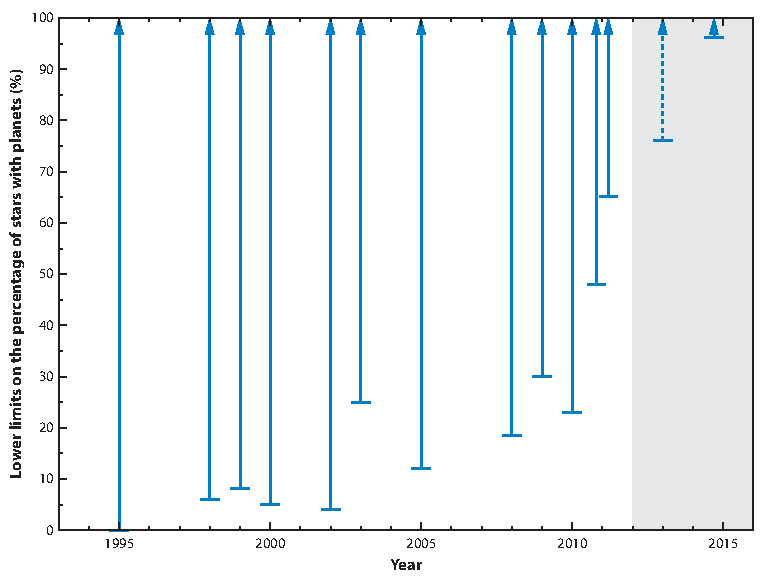
\includegraphics[width=0.9\linewidth]{figures/AnnRevs/AR8.pdf}
	\caption[Fraction of stars with planets]{Lower limits to the fraction of stars with planets as a function of time. Because published values are based on limited ranges in mass or period (\ie, small areas in the parameter space of Figure~\ref{fig:AR9}), they are not estimates of the real fraction of stars with planets but are lower limits. These lower limits have been rising as the durations of surveys increase and detection sensitivity improves. The predicted lower limits at 2013 and 2015, suggesting that 100\% of stars have planets, are based on the trends seen in the past three years and the plausible range over which these trends can be extrapolated}
	\label{fig:AR8}
\end{figure}


%%%%%%%%%%%%%%%%%%%%%%%%%%%%%%%%%%%%%%%%%%
\begin{figure}[!hbt]
	\centering
	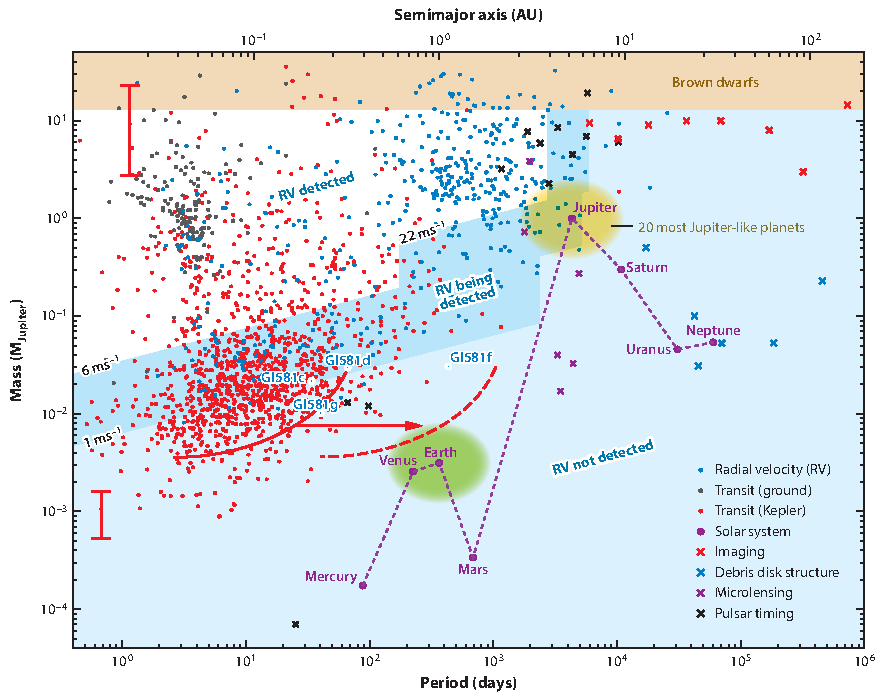
\includegraphics[width=0.9\linewidth]{figures/AnnRevs/AR9.pdf}
	\caption[Exoplanet detection techiques and yeilds]{Our Solar System compared to $\sim$\,1,870 exoplanets detected using various techniques. The region around our planetary system and to the lower right has not been well explored. The red cloud of points in the lower left represents the $\sim$\,1,200 Kepler planet candidates from \citet{Borucki2011}. The other $\sim$\,670 exoplanets were detected by other instruments. After the nominal approximately four-year Kepler mission, the red curve, approximating the limit of the Kepler cloud, will have moved to the dashed red curve. At least a few Earth-mass planets in Earth-like periods around Sun-like stars are expected within the green oval surrounding Earth. If the Sun were removed to some typical distance ($\sim$\,30 light years) and were on the target list of our planet-hunters, it would probably still be listed as having no planets. The yellow oval contains the 20 most Jupiter-like planets, which are plotted separately in Figure~\ref{fig:AR11}. Timothy Bovaird was instrumental in helping to make this figure.}
	\label{fig:AR9}
\end{figure}


Planet detections have technique-dependent limits \citep{Cumming2010}. Figure~\ref{fig:AR9} shows how the eight planets of our Solar System (dashed purple line) compare to the $\sim$\,1,870 exoplanets compiled from six detection techniques listed in the lower right. The estimated masses of the planets are plotted as a function of their orbital periods.

The most important take-home message is: Yes, there are planets around other stars. The second message is that most of the patterns in the data tell us more about instrument sensitivity and survey durations than about the underlying real distribution of planets. Thus, the relatively empty region in the lower right (low mass, long period) appears empty because it has not been well explored. And the blob of dark gray points in the upper left, from ground-based transit searches, is concentrated at high mass and short period because that is where this technique has the highest sensitivity, not because there is a natural concentration of planets there.

The left edge of the red cloud of Kepler points is a real edge due to the underlying distribution of planets and tells us that planets with orbital periods less than a couple of days are rare. The lower right edge of the red cloud (indicated by the red curve) is a result of instrument sensitivity and the duration of observations (only 90 days). At the end of the nominal Kepler mission in 2014, Kepler's region of sensitivity will have extended to the dashed red curve, much closer to the region of Venus- and Earth-like planets.

The background of Figure~\ref{fig:AR9} is color-coded to show the sensitivity of the RV technique to planets orbiting solar-mass stars. The ability of the RV technique to detect planets is 100\% in the white region in the upper left, decreases across the ``RV being detected'' region, and sinks to near 0\% in the ``RV not detected'' region. Thus, in the white ``RV detected'' region, any observed pattern of RV planets (blue dots) is a real pattern and is not due to instrument sensitivity or survey duration. The most obvious pattern is that in the high-mass region (1-10 M$_{Jupiter}$), as periods increase (approaching Jupiter's 12-year period), the number of planets increases dramatically. Thus, Jupiter-mass planets become more numerous as we look in more Jupiter-like orbits.

Because the RV technique is most sensitive in the upper left of Figure~\ref{fig:AR9}, Figure~\ref{fig:AR8} is predominantly telling us about the fraction of stars with massive Jupiter-, Saturn-, Uranus-, and Neptune-sized planets that have been scattered or have migrated from their region of formation (farther from the host star) into a region closer to their host star where they could be detected with the RV technique. However, we are more interested in exoplanets that are more similar to Earth in both mass and period. In Figure~\ref{fig:AR9}, planets indicated by the red Kepler dots are the most similar to Earth in mass. If the fraction of stars with large planets is $\sim$\,100\%, what about the fraction of stars with low-mass rocky planets like Earth\,? Based on extrapolation of RV data, \citet{Howard2010} report ``23\% of stars harbor a close-in Earth-mass planet (ranging from 0.5 to 2.0 Earth masses).'' \citet{Wittenmyer2011} report 17\% for planets with mass less than $\sim$\,13 M$_{Earth}$.

%%%%%%%%%%%%%%%%%%%%%%%%%%%%%%%%%%%%%%%%%%
\begin{figure}[!hbt]
	\centering
	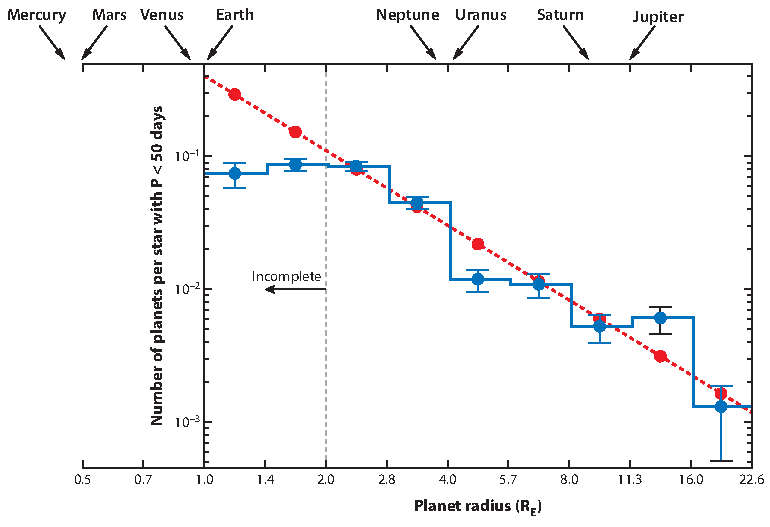
\includegraphics[width=0.9\linewidth]{figures/AnnRevs/AR10.pdf}
	\caption[Kepler results]{Kepler results (as per 2012). The amplitude of the red line tells us that there are many planets close to stars (P < 50 days; for comparison, P$_{Mercury}$ = 88 days). The slope of the red line tells us that there are approximately ten times as many Earth/Venus-sized planets as there are Uranus/Neptune-sized planets and approximately ten times as many Uranus/Neptune-sized planets as there are Jupiter-sized planets. Figure modified from the top panel of Figure~\ref{fig:AR6} in \citet{Howard2012}.}
	\label{fig:AR10}
\end{figure}

Catalogs of exoplanet detections can be found in \citet{Schneider2011} and \citet{Wright2010}. The Kepler planet candidates are from \citet{Borucki2011}. The radii of Kepler candidates have been converted to masses using the average radius-dependent density of the dozen or so least massive exoplanets detected by the transit and radial velocity techniques. Representative uncertainties on this conversion are given in Figure~\ref{fig:AR9} by the size of the vertical error bars on two red points on the far left.

The radii of planets can be extracted from small dips in Kepler's precision photometry of $\sim$\,150,000 stars. Figure~\ref{fig:AR10} is a recent result \citep{Howard2012}. As the fraction of stars with planets approaches its maximum value of 100\% (Figure~\ref{fig:AR8}), this fraction becomes uninformative about the average number of planets per star, which is the y-axis in Figure~\ref{fig:AR10}. The two bins in the region to the left of the dashed gray line (1 < R < 2 R$_{Earth}$) are incomplete because planets that small are harder to detect and need to transit more times for their signal to emerge out of the noise. These incomplete bins were not used to produce the red dashed fit. 

On the left side of Figure~\ref{fig:AR10} notice that the dashed red line crosses R = R$_{Earth}$ at 0.4 planets per star. Because there are many more single-planet stars than multiple-planet systems in the Kepler database, this 0.4 means that $\sim$\,35\% of stars are expected to have planets with radii 0.8 < R < 1.2 R$_{Earth}$ and with orbital periods P < 50 days. That is a large fraction for such a small range of radii and periods. Adding up the values of the red points for the entire range of radii yields the average number of planets (with radii 1 < R < 23 R$_{Earth}$ and P < 50 days) per star: 0.6. When converted to the fraction of stars with a planet, this becomes the 48\% plotted in Figure~\ref{fig:AR8}. Adding up only the values for rocky planets (the three bins with radii 1 < R < 2.8) yields more than 0.5 rocky planets per star. This high frequency within such a small region close to the star (< 0.25 AU) indicates that rocky planets are extremely common.

After Kepler detects more planets with R\,$\approx$\,R$_{Earth}$, if the trend of the red line accurately describes the next smaller bin, the vast majority (perhaps 90\%) of planetary systems may be found to have an Earth-size planet with an orbital period P < 200 days. With Venus's 224-day orbital period and radius R = 0.95 R$_{Earth}$, and Mercury's P = 88 days and R = 0.38 R$_{Earth}$ (too small to detect), such a high observed frequency of close-in exoplanets would make our planetary system unusual for having relatively fewer Earth-sized planets, or having them unusually distant from the host star, or both.

The data collected in Figures \ref{fig:AR8} and \ref{fig:AR9} illustrate that as stars are monitored for longer periods of time, and as we extend our detection sensitivity to Jupiter-like periods, we detect more planets and require less extrapolation to reach the conclusion that $\sim$\,100\% of stars have massive planets. In addition, as we extend our observations to smaller planets (left side of Figure~\ref{fig:AR10}, 0.5 < R < 2 R$_{Earth}$) the numbers increase and again suggest that $\sim$\,100\% of stars have at least one Earth-sized planet.

Other evidence that the fraction of stars with planets is $\sim$\,100\% is that protoplanetary accretion disks are ubiquitous in young star clusters. The observed fraction of young stars with protoplanetary disks approaches 100\% for star-forming regions less than $\sim$\,0.5 million years old \citep{Mamajek2009,Fedele2010}. Also, there are no large planets without a retinue of rocky/icy moons. Many of the moons of Jupiter, Saturn, Uranus, and Neptune are part of miniature planetary systems formed from their planet's miniature accretion disk. ``Planets around every star. Moons around every large planet'' is probably the most reasonable position from which to ponder habitability. Soon we will have detected so many Earth-like planets that our efforts will have to be focused on determining which ones are the most habitable \citep{Horner2010}.

\clearpage

\begin{flushright}
	\textit{If they be inhabited, what a scope for folly;\\if they not be inhabited, what a waste of space.\\
		--- Thomas Carlyle}
\end{flushright}

\section{Circumstellar Habitable Zones}\label{sec:HabitableTemperatures}
Exoplanet research is moving beyond counting planets and plotting their masses and orbital periods. We are beginning to study their temperatures, densities, compositions, tectonic regimes, atmospheric chemistries, and albedos-all factors that can influence habitability. Figure~\ref{fig:AR11} shows that there are several dozen known planets in circumstellar HZs. The least massive are three to five times the mass of Earth. Because the mass of moons seems to scale with the mass of the host planet, the most massive planets in the HZ could harbor habitable moons.

%%%%%%%%%%%%%%%%%%%%%%%%%%%%%%%%%%%%%%%%%%
\begin{sidewaysfigure}[!hbt]
	\centering
	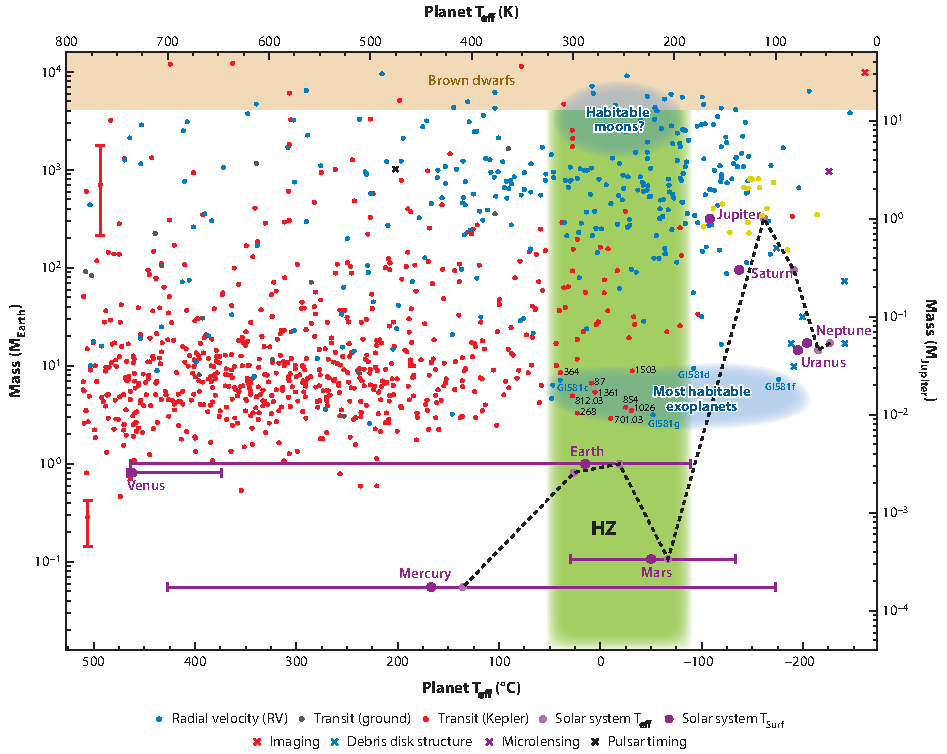
\includegraphics[width=0.65\linewidth]{figures/AnnRevs/AR11.pdf}
	\caption[Planets in the circumstellar habitable zone]{Planet temperatures and the circumstellar habitable zone (HZ). This figure is essentially the same as Figure~\ref{fig:AR9} except we have used our knowledge of the luminosity of the host stars to convert orbital periods into effective temperatures (T$_{effective}$) at the planet's distance from its host. To obtain T$_{effective}$ values for exoplanets and the planets of our Solar System in the same way, we have followed the appendix of \citet[][version 1 only, but using albedo\,=\,0.3, $\varepsilon$\,=\,1, $\beta$\,=\,1]{Borucki2011}. Because we are trying to evaluate the habitability of exoplanets for which we have only T$_{effective}$ values (not actual surface temperatures), we have shifted the habitable temperature range (+122\textcelsius{} to -20\textcelsius{}) by 80\textdegree{} (keeping the 144\textdegree{} width) to be centered on the T$_{effective}$ of Earth. This allows for a more direct comparison of the HZ with exoplanet T$_{effective}$ values and is the simplest way to make a first-order minimal correction for the poorly known extent of exoplanet greenhouse gases and albedos. Because the planets of our Solar System orbit the same star, the dashed lines connecting their (M, T$_{effective}$) coordinates here mirror the dashed lines in Figure~\ref{fig:AR9} connecting their (M, P) coordinates. This is not the case in general. For example, the most Jupiter-like planets (within the yellow oval in Figure~\ref{fig:AR9}) are indicated here with yellow dots. Timothy Bovaird was instrumental in helping to make this figure.}
	\label{fig:AR11}
\end{sidewaysfigure}

For each planet in our Solar System (Figure~\ref{fig:AR11}), notice the difference between the computed effective temperature (T$_{effective}$, small light purple dots) and the actual surface temperatures T$_{Surface}$ (larger purple dots). We have plotted error bars around T$_{Surface}$, indicating the range of surface temperatures on Mercury, Venus, Earth, and Mars. Because $\bigtriangleup${T}{=}T$_{Surface}${-}T$_{effective}$ {>} 0 for all eight planets of our Solar System, all experience some kind of warming.

For Earth we have $\bigtriangleup$T$_{Earth}$ = 33\textdegree, but the thick 90 bar Venutian CO$_{2}$ atmosphere produces $\bigtriangleup$T$_{Venus}$ = 440\textdegree. The variation of $\bigtriangleup$T values within our Solar System is large: 15\textdegree < $\bigtriangleup$T < 440\textdegree, due to differences in albedos and greenhouse gas (CO$_{2}$, H$_{2}$O) column densities. This range gives us an idea of the expected range of exoplanet $\bigtriangleup$Ts that will shift exoplanets to the left in Figure~\ref{fig:AR11}. Thicker atmospheres provide more greenhouse warming and larger $\bigtriangleup$Ts \citep{Marcus2010}. Because we expect $\bigtriangleup$T$_{Super-Earths}$ > $\bigtriangleup$T$_{Earth}$, the shift of the HZ to be centered on the T$_{effective}$ of Earth represents a minimal correction. Thus super-Earths, such as Gl581d just to the right of the HZ, should be considered the best candidates for habitable planets.

A reasonable assumption is that super-Earths (3 < M < 10 M$_{Earth}$) are probably endowed with a mass of greenhouse gases, Mg, proportional to the mass of the planet, M: M$_{g}$ $\sim$\, M. Thus, the column density $\sum$ responsible for greenhouse warming would be $\sum$ $\sim$\, M$_{g}$/surface area $\sim$\, M/R$^{2}$ $\sim$\, R $\sim$\, M$^{1/3}$. With this plausible scaling we would expect the $\bigtriangleup$Ts of super-Earths to be, very roughly, twice as large as the $\bigtriangleup$Ts of our Solar System's planets. Thus, it may be that the half-dozen planets in the middle and left side of the most habitable exoplanets region of the HZ of Figure~\ref{fig:AR11} are greenhouse heated too far to the left to support life.

Gliese 581 is an M star approximately 20 light years away, with a mass M = 0.31 M$_{Sun}$ and $\sim$\,1\% of the Sun's luminosity. Gliese 581's planetary system contains several rocky planets whose habitabilities are being debated \citep{Udry2007,Selsis2007,vonBloh2007,Mayor2009,Wordsworth2011}. The system contains four confirmed planets (Gl581b, -c, -d, -e) and possibly two more unconfirmed planets (Gl581f, -g) \citep{Vogt2010}. With poor signal to noise at the edge of RV sensitivity, the fitted eccentricities can vary between 0 and as much as 0.4. Of the four confirmed planets, Gl581d looks like the best current candidate for being a rocky habitable planet (see also \citep{Kaltenegger2011b}. Its mass is 10$^{{+}4}_{{-}3}$M$_{Earth}$. It receives 35\% less stellar energy than Mars, and its orbital eccentricity is $\sim$\,0. Its period is $\sim$\,66 days and it is tidally locked. It has a radius of $\sim$\,2 REarth, and its surface gravity is approximately twice that of Earth's. Using a global climate model designed for exoplanets, with CO$_{2}$ and H$_{2}$O as greenhouse gases, \citet{Wordsworth2011} find that the range of possible atmospheric pressure is 5-30 bars.

The importance of Gl581 is based on the proximity of its planets to its circumstellar HZ. \citet[][ch 10]{Kasting2012} gives an informed review of the history of the circumstellar HZ and discusses the details of the most cited HZ paper, \citet{Kasting1993}. For details of how the inner and outer limits of the circumstellar HZ are computed, see \citet{Forget1997} and \citet{Abe2011}. The idea of a circumstellar HZ is based on the scenario of surface life kept warm and powered by stellar photons. In the context of the present Earth, this is a reasonable scenario because solar photons control the temperature of the ocean and the top few meters of the continental crust and power most of current life (Figure~\ref{fig:AR4}). But Earth's AHZ may not have been powered by the Sun. If life emerged from a dark hydrothermal vent, vent redox chemistry and the plate tectonic regime that drives it may have more to do with whether life can emerge on a planet than whether the planet is in the circumstellar HZ and has liquid water on its surface. Moving beyond the circumstellar HZ, planets not bound to any star, drifting around between the stars, seem to be the abundant remnants of the gravitational free-for-all in the earliest stages of planet formation in dense star clusters. Using microlensing observations \citet{Sumi2011} report nearly twice as many unbound Jupiters as there are main sequence stars in the galaxy. If there are super-Earths among them with enough hydrogen in their atmospheres \citep{Pierrehumbert2011}, and if life can emerge and persist without photons from a star, then there may be no outer limit to the circumstellar HZ. There may be life-sustaining planets in interstellar space \citep{Stevenson1999}.

\section{Water and Temperature}\label{sec:WaterDel}
Because life as we know it is water-based carbon chemistry, the processes that control the supply of water and carbon to a planet control its habitability. Water is also essential to aid the continual tectonic reworking and erosion that supply key redox gradients and biochemical substrates to sustain habitability (Table \ref{tab:energycurreny}; \citep{Nisbet2007}. \citep{Morbidelli2000} and \citet{Mottl2007} summarize our understanding of the origin of water on Earth. D/H ratios \citep{Robert2001} and much other evidence suggest that the sources of terrestrial water were hydrous bodies such as carbonaceous chondrites (5\%–20\% water) from the outer part of the main asteroid belt. An alternative wet accretion model has between one and three oceans of water accreting with the planetary embryos that formed the bulk Earth \citep{Drake2002, Drake2005}. A third possibility discussed by \citet{Mottl2007} is the acquisition of hydrogen and water directly from the solar nebula by adsorption onto accreting material and dissolution into a magma ocean.

Because variations in temperature and water content are the two most important variables in delimiting the habitability of Earth, they should be the basis of any classification scheme for the habitability of planets. The green circumstellar HZ in Figure~\ref{fig:AR11} is based on effective temperature computed from stellar type and semimajor axis. To obtain more accurate surface temperatures, we need to know more about planetary greenhouse gas content and albedos. The amount of water on a rocky planet can depend on the C/O ratio of the star (because C/O controls the amount of water in the protoplanetary disk), but like T$_{Surf}$, water content depends on many variables. Numerical simulations that take into account the notionally most important parameters indicate that water content on a terrestrial planet can vary typically by factors of a few \citep{Raymond2007} and probably much more (perhaps an order of magnitude) when more parameters are allowed to vary. Variations in water supply are caused by variations in the number of impacts with water-rich planetesimals. The number of impacts is a function of planetary position (proximity to the snowline) and planetary mass (to gravitationally focus the impactors). Impacts also depend on the mass, eccentricity, and orbital evolution of the Jupiter analog in the system (if there is one) \citep{Levison2003,OBrien2006}.

\begin{table}[tbh]
	\centering
	\caption{Planet classification according to water content}
	\resizebox{\textwidth}{!}{
	\begin{tabular}{@{}lcc@{}}
		\toprule
		{Name}     & {\% surface} & {Features}\\ 
		   & {liquid water} & \\ \midrule
		Ocean planet      &  $\sim$\,100\%                           & Hydrothermal vents, little erosion \citep{Kuchner2003,Leger2004}\\
		Earth-like planet & 1\%-99\%                         & Continental and oceanic crust, surface erosion, fresh water\\
		Desert planet     &  $\sim$\,0\%                             & Wider habitable zones\,?  \citep{Abe2011}\\ \bottomrule
	\end{tabular}
	}
		\label{tab:planetclassification}
\end{table}

\begin{table}[tbh]
\caption{Planet classification according to water content}

\label{tab:planetclassification2}
\centering
\begin{footnotesize}
\rowcolors{3}{tableShade}{white} %% start alternating shades from 3rd row
\begin{tabular}{cll}
\toprule
\hiderowcolors 
\tabhead{Name} & \tabhead{\% surface} & \tabhead{Features}\\
 & \tabhead{liquid water} & \\
\midrule
\showrowcolors
Ocean planet      &  $\sim$\,100\%                           & Hydrothermal vents, little erosion \citep{Kuchner2003,Leger2004}\\
		Earth-like planet & 1\%-99\%                         & Continental and oceanic crust, surface erosion, fresh water\\
		Desert planet     &  $\sim$\,0\%                             & Wider habitable zones\,?  \citep{Abe2011}\\ \bottomrule
\end{tabular}
\end{footnotesize}
\end{table}

Another complication is that Earth may have acquired far more water during its formation than exists in its ocean and mantle today \citep{Abe2000}. Variations in the ability of a planet to hold onto the supplied water depend on planetary mass, temperature (through thermally induced hydrodynamic escape), atmosphere, the amount of collisional erosion \citep{Genda2005,ONeill2008}, and the degree of differentiation of the impacting planetesimals. In the first few million years, $^{26}$Al (half-life 0.7 million years) provides much of the radiogenic heat (in addition to the heat of accretion) responsible for the density segregation of planetesimals, exposing water on the outside while sequestering iron on the inside \citep{Grimm1993,Hester2005}. Importantly, the $^{26}$Al content of a protoplanetary disk can vary by several orders of magnitude since it depends on how close the disk is to the closest supernovae produced by the largest stars in the birth cluster \citep{Bizzarro2004,Gaidos2009,Gilmour2009,Adams2010}. Because of the large variation possible in the water content of rocky planets, it makes sense to classify them by water content and by the phase of that water (solid, liquid, or gas) (see Table \ref{tab:planetclassification}). 


Ocean, Earth-like, and desert planets will each have low-, moderate-, and high-temperature versions. For example, a low-temperature ocean planet will be covered with ice (Europa-like), possibly because it is too small to maintain ongoing volcanism, or too poor in the four long-lived radiogenic isotopes to recover from episodes analogous to snowball Earth \citep{Hoffman2002}. A high-temperature version of an ocean planet would be a steam planet. Desert planets, low in H$_{2}$O owing to a small amount of radial mixing of material beyond the snowline, would also be low in carbon. Low carbon could also be a factor limiting the habitability of planets orbiting stars with low C/O ratios. See \citet{Bond2010} and \citet{Delgado-Mena2010} for a discussion of how stellar variation in C/O and Mg/Si can affect the mineralogy and habitability of rocky planets. For example, they find that stars with C/O > 0.8 will host reduced carbide planets with little water.

\clearpage
\section{The Galactic Habitable Zone}\label{sec:GHZ}

Life is embedded in a hierarchy of supporting environments that provide the requirements for habitability. Estimation of a circumstellar HZ assumes the presence of a star and a planet and addresses the question, Where can the planet be located such that its surface is at the right temperature for life\,? The galactic HZ is a similar idea but on a much larger scale: Given an 11-billion-year-old galaxy, where can you find a star, a rocky planet, and clement conditions that last long enough to maintain life\,? The idea of a galactic HZ was intimated by  \citet{Lem1986}, clearly articulated by \citet{Gonzalez2001}, extended and more carefully quantified by \cite{Lineweaver2004} (Figure~\ref{fig:AR12}), and refined spatially to individual stars in a Monte Carlo simulation by \citet{Gowanlock2011} \citep[see however,][]{Prantzos2008}. Stars in our galaxy are not distributed uniformly in either space or time, nor do they all have enough metallicity (elements excluding H, He) to accrete rocky planets. And some are dangerously close to supernovae that disrupt habitability. \citet{Lineweaver2004} mapped the distribution in space and time of four prerequisites for complex life: the presence of a host star, enough heavy elements to form terrestrial planets, sufficient time for biological evolution ($\sim$\,4 billion years), and an environment free of life-extinguishing supernovae. We identified the galactic HZ as an annular region between seven and nine kiloparsecs from the galactic center that widens with time and is composed of stars that formed between eight and four billion years ago. Similar to the boundaries of the circumstellar HZ, these limits are not sharp, but do indicate where the potential for complex (= 4 billion years old) life may be the highest. This galactic HZ yields an age distribution for the complex life that may inhabit our galaxy: 75\% of the stars in the galactic HZ are older than the Sun.

%%%%%%%%%%%%%%%%%%%%%%%%%%%%%%%%%%%%%%%%%%
\begin{figure}[!hbt]
	\centering
	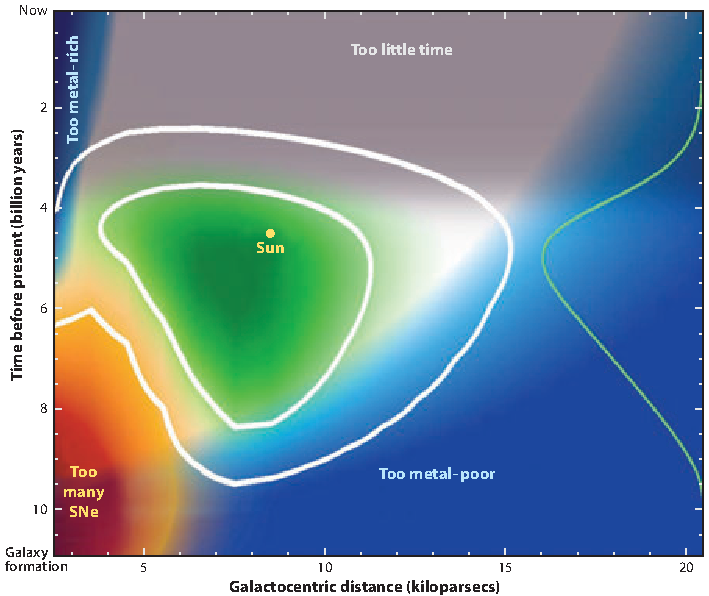
\includegraphics[width=1\linewidth]{figures/AnnRevs/AR12.pdf}
	\caption[Galactic habitable zone]{Galactic habitable zone (HZ) of our Milky Way Galaxy from \citet{Lineweaver2004}. ``Too many SNe'' indicates the region where the supernovae (SNe) rate is probably too high to be compatible with the evolution of life.}
	\label{fig:AR12}
\end{figure}

Stars in our galaxy are not distributed uniformly in either space or time, nor do they all have enough metallicity (elements excluding H, He) to accrete rocky planets. And some are dangerously close to supernovae that disrupt habitability. \citet{Lineweaver2004} mapped the distribution in space and time of four prerequisites for complex life: the presence of a host star, enough heavy elements to form terrestrial planets, sufficient time for biological evolution ($\sim$\,4 billion years), and an environment free of life-extinguishing supernovae. We identified the galactic HZ as an annular region between seven and nine kiloparsecs from the galactic center that widens with time and is composed of stars that formed between eight and four billion years ago. Similar to the boundaries of the circumstellar HZ, these limits are not sharp, but do indicate where the potential for complex (= 4 billion years old) life may be the highest. This galactic HZ yields an age distribution for the complex life that may inhabit our galaxy: 75\% of the stars in the galactic HZ are older than the Sun.

One can extend the concept of HZ beyond the galaxy to the universe. For example, a cosmic temporal HZ can be constructed from the age distribution of terrestrial planets in the universe \citep{Lineweaver2001}. There are times that are habitable and times that are not. In the first two to three billion years after the big bang, there were no terrestrial planets because there was not enough condensable material to make them. There are also many other features of our universe that play a role in its habitability. These are discussed insightfully elsewhere \citep{Dicke1961,Carter1974,Barrow1988,Bostrom2002,Carroll2006,Barrow2006}.

Following \citeauthor{Lovelock1965}'s \citeyear{Lovelock1965} idea that the simultaneous presence of oxygen and reduced gases (\eg~CH$_{4}$, H$_{2}$) is unlikely without life, \citet{Sagan1993} analyzed a spectrum of Earth taken by the Galileo probe, searching for signatures of life. They concluded that the large amount of O$_{2}$ and the simultaneous trace amounts of CH4 are strongly suggestive of biology. This has been a model of how we might be able to remotely detect life elsewhere \citep{Leger1999}. However, oxygen can be produced abiotically by photolysis of water with subsequent hydrogen escape and photolysis of CO$_{2}$ with subsequent burial of carbon. The future search for extraterrestrial life will rely on our improved ability to understand and spectrally characterize the abiotic and potentially biotic contributions to atmospheric chemical disequilibria \citep{Kasting2009,Krissansen-Totton2016,Seager2010,Vazquez2010,Kaltenegger2011b}.

The study of habitability, \textit{habitology}, is a new, cross-disciplinary synthesis of facts and theory from Earth and planetary sciences, biology, and astronomy. As new data come streaming in from these disparate disciplines, the preliminary steps of their integration is exhilarating and confusing. We can only find out who we are and how we fit into the universe by studying and interpreting these data with the goal of finding other life-forms. Our search for extraterrestrial life is a search for ourselves and our place in the universe. If we cannot find extraterrestrial life-forms that fit our definition of life, perhaps we will have to broaden our definition until we do. Even if we fail to find life elsewhere, we will soon find the closest uninhabited habitable planet. That will be crucial, sooner or later, for our survival as a species.